\scanpage{5}
\mspage{2)}
\figure{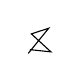
\begin{tikzpicture}[scale=.4]\draw (0,0)--(.65,.8)--(.1,.62)--(.72,.05)--(.05,.12);\end{tikzpicture}}
\[
T\subset S\supset U=S-T
\]
\margin{\figure{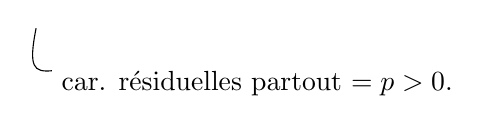
\begin{tikzpicture}\node[anchor=west] at (.2,0) {car. résiduelles partout $=p>0$.};\draw (0,.7) .. controls (-.1,.2) and (-.03,.14) .. (.2,.16);\end{tikzpicture}}}
\margin{\unsure{3.}}
\[
A\longmapsto (A_U,T_p^{\unsure{f|p}}(A),\varphi)
\]
schémas abéliens sur $S$ \qquad triples $(A_U,M,\varphi)$
\[
\begin{aligned}
&A_U\quad\text{schém. abélien sur }U\\
&M\quad\text{\unsure{grpe} $p$-div sur }T\\
&\varphi:T_p^{\unsure{f|p}}(A_U)\simeq M.
\end{aligned}
\]
\margin{$S$ noethérien, $U$ \deleted{dense} \deleted{\unsure{schémati.}} \deleted{\uline{\unsure{schématiquement}}} dense et $S-U$ à car. $p$.}
\margin{\figure{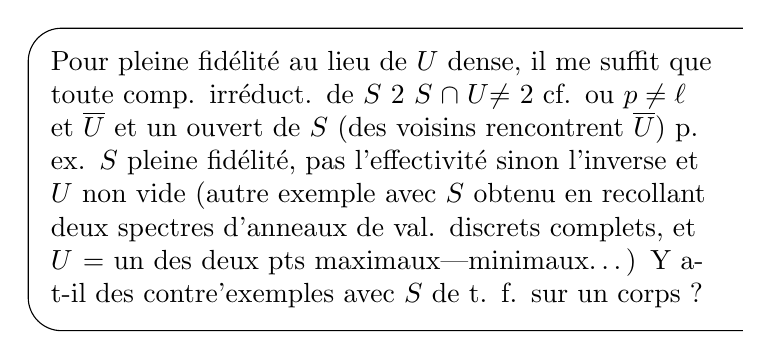
\begin{tikzpicture}\node[inner sep=8pt,text width=8.5cm] (n) {Pour pleine fidélité au lieu de $U$ dense, il me \unsure{suffit que} \deleted{\unsure{toute} comp. \unsure{irréduct.}} \deleted{\unsure{de $S$} \illegible{2} $\unsure{S}\cap U\unsure{\ne}\varnothing$ \illegible{2}} \deleted{\unsure{cf. ou} $\unsure{p\ne\ell}$} \deleted{et $\overline U$ \unsure{et un ouvert} de $S$ (\unsure{des voisins} \unsure{rencontrent} $\overline U$)} p. ex. $S$ \deleted{\unsure{pleine fidélité}, \unsure{pas l'effectivité}} \unsure{sinon l'inverse et $U$ non vide} (autre exemple \unsure{avec} \unsure{$S$} obtenu en \unsure{recollant} deux spectres d'anneaux de val. discrets complets, et $U=$ un des deux pts \unsure{maximaux|minimaux}\dots) Y a-t-il des contre'exemples avec $S$ de \unsure{t. f.} sur un \unsure{corps} ?};\draw[rounded corners=12pt] (n.north east)--(n.north west)--(n.south west)--(n.south east);\end{tikzpicture}}}

1) \uline{Foncteur pleinement fidèle}

fidèle bien connu, car $A\mathbin{-}T_p^{\unsure{f|p}}(A)$ est fidèle.

``pl.'' fidèle: il faut prouver que si $u_p:T_p^{\unsure{f|p}}(A)\mathbin{-}T_p^{\unsure{f|p}}(B)$ est algébrique sur $U$, il l'est sur $S$. Si $U$ est sch. dense dans $S$, cela résulte de $[\ ]$ 1.2. Dans le cas général, soit $X_0$ l'adhérence schématique de $U$ dans $X$.
Alors on dispose d'un hom $\varphi_0:A_{X_0}\to B_{X_0}$, \deleted{\unsure{On voit}} \inserted{compatible avec $u_p$.}

\deleted{Soit $\unsure{I}$ l'idéal qui définit $X_0$ en $X$, \unsure{est nilpotent} \unsure{et} \unsure{s'annule} sur $T$. Alors la \unsure{th.rie} de Serre-Tate implique que l'on peut prolonger la restriction de $\unsure{u_0}$ à $T_0^{\deleted{\unsure{\mathrm{r\acute ed}}}}$ \inserted{$=T$} (muni de la structure induite réduite) en un hom. $A_{T_n}\to B_{T_n}$, où $T_n$ est le $n$-ième voisinage infinitésimal. Se ramenant au cas $S$ affine, \inserted{$=\operatorname{Spec}\Lambda$} on trouve \deleted{\unsure{par l'\illegible{1}}} un hom $A_{\hat\Lambda}\mathbin{-}B_{\hat\Lambda}$, $\hat\Lambda=$ complété de $\Lambda$ pour la top. définie par l'idéal de $T_0$ dans $S_0$. Comme l'hom \deleted{$U\times\unsure{\operatorname{Spec}}$} $\hat\Lambda\to\operatorname{Spec}\Lambda$ est fid plat, on gagne\dots}
\inserted{en appliquant alors $[\ ]$ 1.1.}
\mspage{4}
